\subsection{Validazione e collaudo}
\textit{\textbf{Periodo}: dal 2021-04-23 al 2021-05-26}

L'inizio di questa fase coincide con data della Revisione di Qualifica e si conclude con la scadenza della Revisione di Accettazione.

\subsubsection{Attività}

\begin{itemize}
\item \textbf{Incremento e verifica documenti}: vengono realizzati gli incrementi necessari ai documenti. I documenti in questione sono:
\begin{itemize}
\item \NdP{};
\item \AdR{};
\item \PdQ{};
\item \PdP{};
\item Glossario;
\item \MU{};
\item \MM{}.
\end{itemize}
\item \textbf{Validazione e collaudo}: viene completato il prodotto e i documenti in base a requisiti mancanti, indicazioni del proponente o analisi interne. Vengono inoltre eseguiti tutti i test per validare e collaudare il prodotto finale.
\item \textbf{Consolidamento}: viene realizzata la presentazione da esporre in sede di Revisione di Accettazione.
\end{itemize}

\subsubsection{Incremento 11}
\myparagraph{Consuntivo}

{

\rowcolors{2}{azzurro2}{azzurro3}

\centering
\renewcommand{\arraystretch}{1.8}
\begin{longtable}{C{4cm} C{1.5cm} C{4cm} }

\rowcolor{azzurro1}
\textbf{Ruolo} &
\textbf{Ore}&
\textbf{Costo}\\
\endhead

\textit{Responsabile} & 5 (+0) & 150 (+0\euro{}) \\
\ammProg & 6 (+0) & 120\euro{} (+0\euro{}) \\
\analProg & 0 (+0) & 0\euro{} (+0\euro{}) \\
\progetProg & 11 (+0) & 242\euro{} (+0\euro{}) \\
\programProg & 13 (+2) & 195\euro{} (+30\euro{}) \\
\verifProg & 16 (+0) & 240\euro{} (+0\euro{})\\
\textbf{Totale Preventivo} & \textbf{51} & \textbf{947\euro{}} \\
\textbf{Totale Consuntivo} & \textbf{53} & \textbf{977\euro{}} \\
\textbf{Differenza} & \textbf{+2} & \textbf{+30\euro{}} \\


\rowcolor{white}
\caption{Consuntivo di periodo dell'incremento 11}\\

\end{longtable}
}

\myparagraph{Considerazioni}
In questo incremento sono state implementate le ultime funzionalità previste per il nostro prodotto, che ha però portato ad un ritardo e un impegno maggiore di quanto previsto. In particolare sono state trovate alcune problematiche nello sviluppo delle pagine statiche incrementali e nell'autenticazione delle API\ped{G}, ma che sono state risolte tramite ricerche\\
Nonostante ciò, la produzione degli incrementi documentali è risultata come prevista inizialmente.
Dato il ritardo di completamento di questo incremento ed una discussione sugli impegni individuali dei componenti del gruppo durante la fase corrente, è stata effettuata una ripianificazione temporale degli incrementi successivi, lasciando comunque invariato l'impegno orario. Rimangono invariati gli obiettivi dei successivi incrementi.



\myparagraph{Preventivo a finire}
Il bilancio risulta leggermente negativo rispetto al preventivo dell'incremento, con una perdita di 30\euro{}. Esso viene però sanato dal risparmio precedente di 36\euro{}, risultando in un risparmio totale di 6\euro{}.\\ 
Date le considerazioni precedenti e con il bilancio totale ancora in positivo, riteniamo di essere in linea con il preventivo e non prevediamo cambiamenti drastici di esso.


\subsubsection{Incremento 12}
\textit{\textbf{Periodo}: dal 2021-04-30 al 2021-05-08}

\myparagraph{Obiettivi}
Gli obiettivi definiti per questo incremento sono i seguenti:
\begin{itemize}
\item implementazione test mancanti;
\item esecuzione test di sistema;
\item incremento della documentazione, con eventuale correzione in base a segnalazione dei committenti.
\end{itemize}

\myparagraph{Attività}
Per raggiungere gli obiettivi, vengono svolte le seguenti attività:
\begin{itemize}
\item \textbf{codifica}: 
\begin{itemize}
\item implementazione ulteriori test mancanti;
\item correzione di eventuali bug.
\end{itemize} 

\item \textbf{verifiche del prodotto}: esecuzione di test di sistema per l'intero prodotto;

\item \textbf{ampliamento documentazione e verifiche}:
\begin{itemize}
\item eventuali correzioni dei documenti segnalati dai committenti;
\item incremento del \MUv{0.1.0} in base ai test effettuati;
\item incremento del \MMv{0.1.0} in base ai test effettuati;
\item incremento del \Glossariov{3.0.0};
\item rilevazione e registrazione di metriche, esiti di verifica e obiettivi di qualità;
\item aggiornamento dei rischi rilevati;
\item calcolo e registrazione del consuntivo di periodo.
\end{itemize}

\end{itemize}
\myparagraph{Diagramma di Gantt}
\begin{figure}[H]
\centering

\centerline{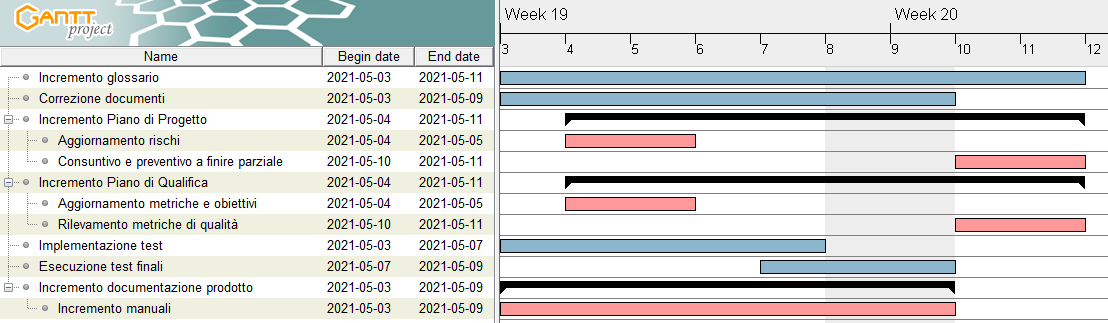
\includegraphics[scale=0.6]{res/Pianificazione/Fasi/VerificaIncrementi/ganttIncremento12}}
\caption{Diagramma di Gantt per l'incremento 12}
\end{figure}
\subsubsection{Incremento 13}
\textit{\textbf{Periodo}: dal 2021-05-09 al 2021-04-17}

\myparagraph{Obiettivi}
Gli obiettivi definiti per questo incremento sono i seguenti:
\begin{itemize}

\item preparazione alla presentazione della Revisione di Accettazione;
\item preparazione al collaudo finale con il proponente;
\item incremento della documentazione.
\end{itemize}

\myparagraph{Attività}
Per raggiungere gli obiettivi, vengono svolte le seguenti attività:
\begin{itemize}
\item \textbf{presentazione Revisione di Accettazione}: creazione e preparazione della presentazione con il \VT{};
\item \textbf{collaudo}: controlli e verifiche ultime al prodotto e ai documenti per il collaudo finale con il proponente;
\item \textbf{ampliamento documentazione e verifiche}:
\begin{itemize}
\item incremento del \Glossariov{4.0.0};
\item rilevazione e registrazione di metriche, esiti di verifica e obiettivi di qualità;
\item aggiornamento dei rischi rilevati;
\item calcolo e registrazione del consuntivo di periodo.
\end{itemize}

\end{itemize}
\myparagraph{Diagramma di Gantt}
\begin{figure}[H]
\centering

\centerline{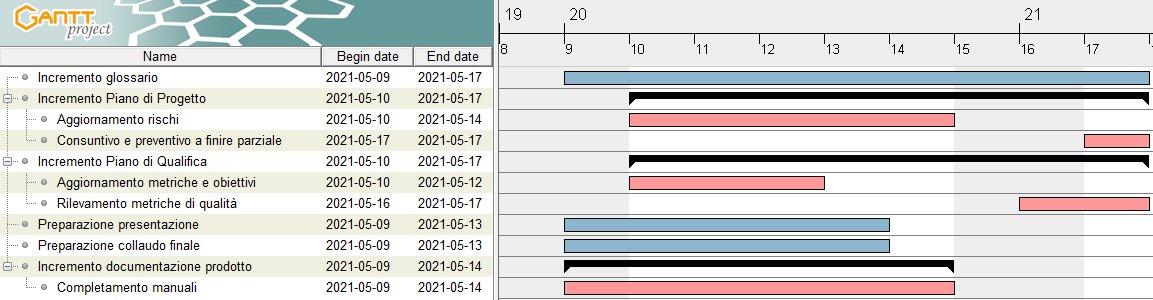
\includegraphics[scale=0.6]{res/Pianificazione/Fasi/VerificaIncrementi/ganttIncremento13}}
\caption{Diagramma di Gantt per l'incremento 13}
\end{figure}